\documentclass[a4paper, 12pt, oneside]{article}


% idioma
\usepackage[utf8]{inputenc}
\usepackage[spanish]{babel}
\usepackage{enumerate}
\usepackage{multirow} % para las tablas
\usepackage{soul}
\usepackage{graphicx}

%tablas
\usepackage{booktabs}

%rotar tablas
\usepackage{rotating}

%color tablas
\usepackage{colortbl}

%espaciado
\usepackage{setspace}
\onehalfspacing
\setlength{\parindent}{0pt}
\setlength{\parskip}{2.0ex plus0.5ex minus0.2ex}


%margenes según n. icontec
\usepackage{vmargin}
\setmarginsrb           { 4.0cm}  % left margin
                        { 3.0cm}  % top margcm
                        { 2.0cm}  % right margcm
                        { 3.0cm}  % bottom margcm
                        {  10pt}  % head height
                        {0.25cm}  % head sep
                        {   9pt}  % foot height
                        { 0.3cm}  % foot sep


% inserción url's notas de pie.
\usepackage{url}

% Paquetes de la AMS:
\usepackage{amsmath, amsthm, amsfonts}

% Paquete para resaltar texto con una caja amarilla para correcciones
\usepackage{color}
\newcommand{\hilight}[1]{\colorbox{yellow}{#1}}

% Teoremas
%--------------------------------------------------------------------------
\newtheorem{thm}{Teorema}[section]
\newtheorem{cor}[thm]{Corolario}
\newtheorem{lem}[thm]{Lema}
\newtheorem{prop}[thm]{Proposición}
\theoremstyle{definition}
\newtheorem{defn}[thm]{Definición}
\theoremstyle{remark}
\newtheorem{rem}[thm]{Observación}

% Atajos.
% Se pueden definir comandos nuevos para acortar cosas que se usan
% frecuentemente. Como ejemplo, aqu se definen la R y la Z dobles que
% suelen representar a los conjuntos de nmeros reales y enteros.
%--------------------------------------------------------------------------

\def\RR{\mathbb{R}}
\def\ZZ{\mathbb{Z}}

% De la misma forma se pueden definir comandos con argumentos. Por
% ejemplo, aqu definimos un comando para escribir el valor absoluto
% de algo ms fcilmente.
%--------------------------------------------------------------------------
\newcommand{\abs}[1]{\left\vert#1\right\vert}

% Operadores.
% Los operadores nuevos deben definirse como tales para que aparezcan
% correctamente. Como ejemplo definimos en jacobiano:
%--------------------------------------------------------------------------
\DeclareMathOperator{\Jac}{Jac}



\newcommand\portada{
\begin{titlepage}
		\begin{center}
			{\large \bf Diseño y prueba de una arquitectura computacional segura para compartir información entre el Hospital del Sur, Instituto Nacional de Salud y la Red de Monitoreo de Calidad del Aire de Bogotá.}
            
			\vfill
 			{\large\bf PRESENTADO POR: \par}
			{\large\bf Marco Antonio Méndez \par}
            {\large\bf Hoffman Antonio Márquez}
			\vfill
			{\large\bf UNIVERSIDAD ANTONIO NARIÑO  \par}
			{\large\bf FACULTAD DE INGENIERÍA DE SISTEMAS \par}
			{\large\bf INGENIERIA DE SISTEMAS Y COMPUTACIÓN \par}
			{\large\bf BOGOTÁ D.C.\par}
			{\large\bf MAYO 16 DEL 2016 \par}
		\end{center}
\end{titlepage}
}

\newcommand\contraportada{
	\begin{titlepage}
		\begin{center}
{Diseño y prueba de una arquitectura computacional segura para compartir información entre el Hospital del Sur, Instituto Nacional de Salud y la Red de Monitoreo de Calidad del Aire de Bogotá.} 
			\vfill
 			{\large\bf PRESENTADO POR: \par}
			{\large\bf Marco Antonio Méndez \par}
            {\large\bf Hoffman Antonio Márquez}
			\vfill
			{\large\bf Anteproyecto de grado \par}
			\vfill
			{\large\bf Directores: Ing. David Alberto Herrera Alvarez PhD. / Ing. Raúl Ernesto Menéndez Mora PhD. 
\par}
			\vfill
			{\large\bf UNIVERSIDAD ANTONIO NARIÑO \par}
			{\large\bf FACULTAD DE INGENIERÍA \par}
			{\large\bf INGENIERIA DE SISTEMAS Y COMPUTACIÓN \par}
			{\large\bf BOGOTÁ D.C.\par}
			{\large\bf MAYO 16 DEL 2016 \par}
		\end{center}
\end{titlepage}
}


%--------------------------------------------------------------------------
% \title{\LARGE \bf Plantilla para un artculo \LaTeX }
% % \vfill
% \author{El autor va aqu\\
%   \small Dept. Plantillas y Editores\\
%   \small E12345\\
%   \small Espaa
% }


\begin{document}
\portada
\contraportada
 

% \abstract{Esto es una plantilla simple para un artículo en \LaTeX.}



\renewcommand\contentsname{\centering TABLA DE CONTENIDOS}
\tableofcontents
\clearpage





%resuelve numeración
\renewcommand{\thesection}{}
\renewcommand{\thesubsection}{\arabic{section}.\arabic{subsection}}
\makeatletter
\def\@seccntformat#1{\csname #1ignore\expandafter\endcsname\csname the#1\endcsname\quad}
\let\sectionignore\@gobbletwo
\let\latex@numberline\numberline
\def\numberline#1{\if\relax#1\relax\else\latex@numberline{#1}\fi}
\makeatother
% fin resuelve numeración

\begin{center}
 \section{RESUMEN}
 \end{center}
 
Los datos e información en la actualidad son un recurso vital para todos los procesos que se llevan hoy en la sociedad ya que los datos son la recopilación de hechos que suceden en todos los ámbitos de la vida cotidiana. En el caso de la investigación es importante la protección e integridad de los datos tanto de organismos públicos como privados. Pero ¿ qué sucedería, sin importar el origen de la información, si pudiera realizar un análisis de los datos de diferentes proveedores para encontrar relaciones o agrupamientos preservando la integridad y protegiendo la información cada proveedor?

El propósito de esta investigación es plantear y aplicar una arquitectura computacional segura que permita realizar procesos de análisis de datos de diferentes proveedores de información de forma privada (anónima), para encontrar resultados que se  hallarían solamente de manera colaborativa entre los proveedores de información.Se realizará un proceso de protección de los datos de cada proveedor a través de procesos de cifrado con el fin de poder realizar un análisis de manera global de información particular. 

El planteamiento de la arquitectura computacional segura se validará a través de tres bases de datos de diferentes proveedores de información, para este caso, de instituciones públicas: el Hospital del sur, la Secretaría de Ambiente de Bogotá y el Instituto Nacional de Salud.

Palabras clave: Arquitectura multi-partita, mienría de datos, encriptación, seguridad informatica.

 \clearpage
 
\begin{center}
 \section{INTRODUCCIÓN}
 \end{center}
 
 Los datos para cada persona u organización son un recurso importante para tomar decisiones, pero  en ocasiones se desea encontrar información que solamente se puede hallar con la colaboración conjunta de diferentes fuentes de información. La privacidad e integridad de los datos de cada proveedor de información se debe preservar en este proceso de compartir los datos para evitar fugas o escape de información delicada o confidencial.Se planteará y probará en la investigación una arquitectura computacional segura para realizar minería de datos con tres proveedores de información diferentes.

Se realizará un proceso de cifrado a cada base de datos privada a través de tecnologías de criptografía con el lenguaje de programación Python. Esto permitirá extraer los datos a una base de datos pública donde se realizará un proceso ETL (extracción, transformación y carga) para poder aplicar la técnica de agrupamiento de minería de datos con el fin de dividir los datos en grupos de objetos. Los métodos de agrupamiento no paramétricos pueden dividirse en tres grupos fundamentales: jerárquicos [1-4], particionales [1] y basados en densidad [5-9].

La arquitectura computacional segura propuesta se implementará en las tres bases de datos de prueba: RIPS (Hospital del Sur Bogotá), Red Monitoreo de Calidad de Aire de Bogotá (Secretaría de Ambiente de Bogotá) y el SIVIGILA (Instituto Nacional de Salud) para encontrar una correlación entre los datos y definir un agrupamiento según las enfermedades de infecciones respiratorias agudas con los registros de contaminación del aire, todo esto sin exponer el origen de cada dato.

\clearpage

\begin{center}
 \section{PLANTEAMIENTO DEL PROBLEMA}
 \end{center}

\subsection{DESCRIPCIÓN DEL PROBLEMA}

Las emergencias por infección respiratoria aguda en el mundo han generado la necesidad de reconocer la importancia de fortalecer la estructura y los procesos de vigilancia de la infección respiratoria
aguda (IRA). Una de las recomendaciones internacionales es la de consolidar la vigilancia sobre este conjunto de enfermedades con un reglamento sanitario, pero a través de estrategias que garanticen una oportuna detección y prevención de estos tipos de emergencias.

Aunque en Colombia se ha realizado seguimiento y notificación de las infecciones respiratorias agudas, se presentan limitaciones de las entidades responsables del sector de salud y ambiental. Entre estas está la dificultad para acceder a la información de cada entidad, ya por procesos burocráticos o razones de confidencialidad, lo que puede dificultar la detección temprana de morbi-mortalidad causado por diferentes agentes etiológicos.

Una estrategia para poder detectar cifras o patrones de morbi-mortalidad de manera más acertada y anticipada es poder acceder a la información de diferentes fuentes, ya que el acceso a los datos podría estar limitado por cada una de estos. Debido a la complejidad y a lo delicado que es manejar esta información, por la cantidad de datos que se encuentran en cada uno de ellos, es importante encontrar un mecanismo tecnológico con el cual se pueda mantener la confidencialidad de la información de cada uno de los datos suministrados por parte de los entes o instituciones publico-privadas.

Existen casos en los que los diferentes métodos de compartir información han causado intentos fallidos y exitosos por protegerlos; uno de estos casos fallidos sucedió en la ciudad de New York en el año 2014, cuando se recopiló la información de todos los taxistas de la ciudad por parte de la alcaldía neoyorkina. Pero una falla en el proceso de cifrado MD5 permitió que personas ajenas recuperaran información personal de los taxistas de alrededor de 173 millones de viajes realizados [10], dejando en evidencia sus datos personales y las rutas con sus clientes frecuentes,  perjudicando así su privacidad. Si esta información la obtuvieran grupos criminales podrían dar seguimiento a taxistas y pasajeros.

Un caso exitoso fue el de Netflix, cuando en el año 2006 logró anonimizar la información de más de 500.000 millones de clientes junto a las preferencias de los mismos, mostrando un grado de nivel alto de seguridad y preservación de la integridad de los datos [11].

Se buscará una solución computacional con la combinación de diferentes técnicas con las cuales sean importante  para poder compartir información entre diferentes entidades. En el caso de la investigación se diseñara un mecanismo para compartir información preservando y protegiendo los datos de los proveedores de prueba. 

\subsection{FORMULACIÓN DEL PROBLEMA}

¿Qué mecanismo tecnológico se puede aplicar para compartir información de manera segura y anónima entre las diferentes entidades con las que se trabajará en dicha investigación ?

\subsection{JUSTIFICACION}

Teniendo en cuenta la problemática y para  poder encontrar una correlación entre los eventos registrados en el Hospital del Sur referente a las infecciones respiratorias agudas, con los hechos meteorológicos y atmosféricos de las tres estaciones de la Red de Monitoreo de Calidad de Aire de Bogotá, se tendrá en cuenta que la información del Hospital del Sur, por ser de caracter médica, debe ser protegida contra procesos o eventos que puedan perjudicar a los pacientes u hospital, por fugas de datos confidenciales. 

Para las base de datos privada (RIPS) del Hospital del Sur será la relevante para proteger su información. Dentro de los procesos internos del hospital, solo se expone al público datos que no son importantes ni sensibles. En el proceso de compartir información con otras bases de datos se sigue el alineamiento de no exponer información confidencial, ya que los datos deben ser anónimos, sin olvidar la integridad original de los registros hospitalarios.

Se tiene en cuenta que las bases de datos de la Secretaría de Ambiente de Bogotá y el Instituto Nacional de Salud no será primordial el anonimato de los datos, sino la integridad de la información, puesto que en estas bases de datos no existe información médica sensible para cohibir su publicación, pero sin que ningún evento corrompa los datos originales. En el proceso de compartir información entre las tres entidades, se tendrá relevancia en la integridad de la información de cada, pero protegiendo la exposición pública de datos registrados en el Hospital del Sur.

Para la proteger el anonimato e integridad de la información, se definirá cada entidad como un proveedor privado, los cuales expondrán parte de los datos en una base pública para un proceso de minería futuro, teniendo en cuenta que aquella información no deberá permitir la identificación de su origen ni afectar las bases de datos originales en caso de corrupción en la información expuesta públicamente.

Se diseñará una arquitectura computacional segura, que permita el proceso colaborativo de las tres entidades, para poder realizar una exposición de información de cada una, preservando los datos originales de manera segura y anónima.

Ya garantizando la integridad y anonimato de la información, se realizará un proceso de prueba de minería de datos, para poder correlacionar los datos del Hospital del Sur con RMCAB a través del método de agrupamiento de datos (Clustering) para encontrar los posibles focos de concentración de población con infecciones de respiración aguda referente a los registros de contaminación del aire. De esta manera, se comparará con la información del SIVIGILA. Los resultados de la minería de datos serán un apoyo  al Hospital del Sur para posibles planes de manejo de prevención de las IRA. Igualmente permitirá realizar informes u otros documentos de manera ágil y económica entre las tres entidades evitando procesos de autorizaciones y burocráticos.

Además un aporte al desarrollo del proyecto para la facultad de Ingeniería de Sistemas y Computación es promover un nuevo campo de investigación de arquitecturas de computación seguras implementando minería de datos con información encriptada. Finalmente, esto en la vida profesional será el inicio para la profundización con la maestría en Seguridad Informática como así mismo en especializaciones en minería de datos.

\subsection{OBJETIVOS}

\subsubsection{Objetivo General}
\begin{itemize}
\item Diseñar una arquitectura computacional que permita compartir información del Hospital del Sur, Instituto Nacional de Salud y la Red de Monitoreo de Calidad del Aire de Bogotá, garantizando la integridad y privacidad de los datos de cada proveedor de información.
\end{itemize}

\subsubsection{Objetivos Específicos}
\begin{itemize}
\item Diseñar una arquitectura computacional segura y adecuada, basada en los diferentes mecanismos de seguridad para el intercambio de información entre los diferentes proveedores de información.
\item Implementar el mecanismo encontrado con las tecnologías apropiadas para el buen funcionamiento de la arquitectura computacional segura.
\item Probar la arquitectura implementada para realizar minería de datos de los proveedores definidos para la investigación (Hospital del Sur, Secretaría de Medio Ambiente y Instituto Nacional de Salud Pública).

\end{itemize}

\subsection{ALCANCE Y LIMITACIONES DEL PROYECTO}

Para hacer un análisis de las infecciones respiratorias agudas, se escogerán los datos relevantes de cada proveedor de información. Cada proveedor cuenta con su  manejo de información definido, el cuál se deberá entender para definir los posibles identificadores que ayudarán en los procesos posteriores de minería de datos. 

Se realizará en cada uno de las bases de datos un proceso de ETL (extracción,transformación y carga) para definir la información requerida para la investigación. Dentro del proceso del ETL, en cada base de datos se definirán los posibles identificadores y cuasi identificadores para clasificarlos en confidenciales y no confidenciales [12], para determinar los algoritmos de extracción.

Los datos extraídos se guardarán en un banco de datos público utilizando un motor de base de datos Postgresql. El diseño de la base de datos pública se da a partir de los datos extraídos para facilitar el proceso de la minería de datos. La base de datos se montará en los equipos de los  investigadores para el desarrollo de los scripts en Python.

En la ejecución de la extracción de la información en cada un de los proveedores privados se debe preservar la privacidad de los datos para realizar la transformación e inserción al banco de datos público. Esto se garantizará mediante la implementación de una arquitectura multi-partita computacional, la que permitirá la interacción entre los agentes de información de manera individual, protegiendo las diferentes estructuras con técnicas aplicadas para este tipo de arquitectura.

Ya implementada la arquitectura multi partita computacional, se utilizará la herramienta RapidMiner para realizar el proceso de minería de datos, utilizando algoritmos de relación ya implementados.

La información de prueba por parte del Hospital del Sur será del año 2015, la cual tendrán los movimientos registrados de hospitalizaciones y consultas médicas, entre otros. Los datos de ese proveedor suministrará edades, nombres, direcciones, nombres de enfermedades de los pacientes, los cuales serán los más relevantes para proteger contra la exposición inadecuada.

De la Red de Monitoreo de Calidad del Aire también se usarán los registros del año 2015 de las siguientes estaciones Kenedy (Carrera 80 Nº 40-55 Sur), Puente Aranda (Calle 10 Nº 65-28) y Carvajal (Autopista Sur Nº 63-40). Este proveedor nos dará registros de estadísticos de los contaminantes y variables meteorológicas.

En cuanto al SIVIGILA, tendremos la información de confirmación de los casos positivos de las infecciones de respiración aguda del año 2015 en la ciudad de Bogotá.

Dentro de las limitaciones de la arquitectura, no se garantizará por completo la protección de los datos contra ataques directos como son inyecciones SQL o sobre carga de información, ya que la arquitectura se enfocará en el intercambio de los datos con técnicas de cifrado sin afectar directamente las bases de datos privadas. 


\begin{center}
\section{METODOLOGÍA}

\end{center}
Como parte de los diferentes métodos de investigación es muy importante definir de manera asertiva cuál aplicar y también cuál de cierta manera aporte de una manera óptima los recursos que serán utilizados para cada una de sus tareas.

Durante la elaboración de estas tareas, la manera en que se realizará el análisis y la síntesis de los procesos es de manera individual partiendo desde un todo  como eje principal. El análisis por el medio del cual una realidad es descompuesta en partes para su mayor compresión, ya que a partir de un todo se pueda estudiar proceso a proceso sin afectar el proceso que las une. 

Como síntesis del comportamiento resultante de su respectivo análisis también partirá granularmente hasta llegar a emplear de esta manera todo una serie de pasos a los que llegara a unir todos y cada uno de sus procesos.

La regla de descomposición aplicada para este método de investigación es de cierta forma la más adecuada debido a la cantidad de información suministrada por parte de las fuentes de información y el proceso que se implementara: análisis exhaustivo de todos los detalles,
comportamientos y características de cada uno de los elementos constitutivos de un todo, y estudio de sus partes.

Finalmente, Clasificación como Ordenación de cada una de las partes por clases, siguiendo el patrón del fenómeno analizado, para conocer sus características, detalles y comportamiento y así mismo llegar a una conclusión entregando un análisis de resultados obtenidos para luego ser estudiados y dar explicación del fenómeno observado.

\begin{enumerate}[I]
\item\textbf{Observación}
%sus hechos, comportamiento, partes y componentes.

Dentro del proceso de identificación de las variables de desarrollo de la investigación, se debe tener en cuenta que se debe estructurar según funcionalidad y objetivo de cada parte del  proceso de compartir información entre diferentes proveedores, en el caso de la investigación del Hospital del Sur, Secretaría de Ambiente de Bogotá e Instituto Nacional de Salud. La identificación de los componentes o partes, se dará por el tipo de objeto o uso, según lo nombrado se entenderá que se clasificará en las siguientes categorías o pilares:

\begin{enumerate}[1.]
\item{Proceso de Información (Proveedores de Información / Bases de Datos)}
\item{Procesos de Seguridad Informática}
\item{Procesos de ETL}
\item{Procesos de Minería de Datos}
\end{enumerate}

\item\textbf{Descripción}
%Identificación de todos sus elementos, partes y componentes para poder entenderlo.
Dentro de la descripción de las categorías definidas anteriormente, se realizará la identificación del comportamiento dentro de la arquitectura como la importancia dentro de la secuencia que se llevará en el desarrollo de la investigación.

\begin{enumerate}[1.]
\item{Proceso de Información (Proveedores de Información / Bases de Datos): En esta categoría se define los elementos, objetos o procesos que se relacionen directamente con los datos a compartir de los proveedores, en este caso se entiende que las bases de datos RIPS (Hospital del Sur), SIVIGILA (Instituto Nacional de Salud) y RMCAB (Secretaría de Ambiente de Bogotá) serán los objetos de estudio, para entender qué datos contienen y las relaciones (Entidad - Relación) para definir los datos para realizar el proceso de extracción de dichas bases de datos privadas a la base de datos pública.}
\item{Procesos de Seguridad Informática: Se definirá las tecnologías y métodos de criptografía y seguridad informática, para aplicar a los datos que se extraerán a la base de datos pública. Aquí se realizará el desarrollo en Python de scripts para realizar la cifrado, transporte y carga de los datos a la bases de datos pública, teniendo en cuenta que el proceso debe ser uni-direccional para garantizar que no se exponga el orígen de los datos.}
\item{Procesos de ETL: Se realiza la extracción de la información suministrada por parte de los entes públicos; posteriormente, transformar esta serie de datos en información que sera filtrada de tal manera que su datos represente verdaderamente valor a  frente a lo que se desarrollará; y finalmente ser cargado de una manera en que se podrá manejar. }
\item{Procesos de Minería de Datos: Se realizara básicamente con el datamining o minería de datos, permitiendo comprender el contenido de un repositorio de datos. Con este fin, se hace uso de prácticas estadísticos. De forma general, los datos son la materia prima bruta. En el momento que los proveedores de información les atribuye algún significado especial pasan a convertirse en verdadera información valiosa que en cierto modo será aprovechada para la investigación.}

\end{enumerate}
\end{enumerate}

\clearpage

\begin{center}
 \section{MARCO DE REFERENCIA}
\end{center}

\subsection{MARCO TEÓRICO}


Las Infecciones Respiratorias Agudas (IRA) constituyen un grupo de enfermedades que se producen en el aparato respiratorio, causadas por diferentes microrganismos como virus y bacterias, que comienzan de forma repentina y duran menos de 2 semanas aproximadamente. Es una de las infecciones más frecuente en el mundo y representa un importante tema de salud pública en nuestro país.  La mayoría de estas infecciones como el resfriado común son leves, pero dependiendo del estado general de la persona pueden complicarse y llegar a amenazar la vida, como en el caso de la neumonía.

En niños menores de 5 años, la causa de la infección en el  95\% de los casos son los virus siendo de buen pronóstico, pero un pequeño porcentaje puede padecer complicaciones como  otitis, sinusitis y neumonía. Unos de los efectos que generan gran impacto a nivel local son  la combustión y efectos de cambio climático. Por esto  gran parte de la ciudad adelanta campañas con las que promueve la mejora de la calidad del aire, que con el tiempo será vital.

Se afirma que en países en desarrollo, del 2 al 3\% de los niños presentan enfermedades como neumonía. En invierno es cuando incrementa más la posibilidad de infección viral y también afecta a las mujeres embarazadas y a personas con enfermedades respiratorias.

En cuanto al proceso inicial de los procesos de extracción, transformación y carga (ETL), esto constituye un aspecto clave para llevar a buen camino la integración de los datos, cuyo principal objetivo es conseguir un óptimo rendimiento en la obtención de datos de calidad, que respondan a las necesidades de la empresa de forma fiable.

Dentro del agrupamiento de los datos almacenados, el objetivo principal es encontrar que los objetos de un grupo sean similares entre sí y diferentes de los objetos de otros grupos, aplicando clusters (Colección de métodos Estadísticos).

Es por esto que tanto los  RIPS, SIVIGILA, RMCAB y demás entes que permitieron la recopilación de esta información serán de vital importancia para toda la investigación llevada a cabo. En cuanto a la contaminación en el aire, como principal eje de este factor de riesgo ambiental, analizar qué impacto tiene localmente (Bogotá D.C). De esta manera se tendrá una interacción entre los datos clínicos y la ejecución de métodos computacionales que arrojarán resultados para obtener una serie de análisis y unas conclusiones luego de su proceso. Componente importante dentro de estos procesos sera el de ETL donde se tendrá en cuenta la agrupación de datos para realizar clasificación de grupos basados en su similaridad. 

De esta manera surge la arquitectura multi-partita computacional o  Secure Multiparty Computation (SMC) que permite que entidades o datasets tengan sus entradas independientes para alimentar procesos intermedios para generar salidas independiente, cuidando la comunicación segura de las entradas [13] pero ademas, permitiendo compartir trozos o subconjuntos de datos autorizados con otros participantes  [14]. Una expectativa en el proceso SMC es la interacción entre las partes que permita una funcionalidad independiente pero relacionada para compartir información de manera segura y protegiendo la confidencialidad de cada dato [15].  

Dentro de la arquitectura multi-partita existe gran variedad de técnicas para garantizar la seguridad en este protocolo, como son circuitos ilegibles (garbled circuits), compartiendo secretos (secret sharing) o cifrado homomórfico (homomorphic encryption) [16]. Así, la preservación de la privacidad se obtendrá aplicando la técnica según se requiera. Dentro de las técnicas nombradas se vincula dentro de una composición de una caja negra aritmética (ABB) [17].

\subsection{ESTADO DEL ARTE}
La contaminación de aire en la ciudad de Bogotá ha sido objeto de varios estudios por diferentes entes, ya que se relacionan directamente con enfermedades respiratorias de los habitantes de la capital. Desde 1997, la ciudad cuenta con una red de monitoreo del aire (RCMAB) para la recolección y análisis de los datos recogidos. Las variables que se tienen en cuenta en la recolección son las meteorológicas y las diferentes concentraciones de los contaminantes para encontrar tendencias referentes a la contaminación. Esta tecnología fue tomada de modelos ya implementados alrededor de mundo; por ejemplo en Ciudad de México se encuentran ubicadas 47 estaciones, Londres 30 estaciones, y Beijing 28 estaciones, las cuales suministra información importante para establecer políticas ambientales y de salud.

El sistema RCMAB utiliza para la medición sensores tipo DASIBI u OPSIS, los cuales se encargan de medir variables  como concentraciones atmosféricas y fenómenos meteorológicos, de las cuales se agrupan de la siguiente manera dada en el cuadro 1.0.

\begin{table}[htbp]
\begin{center}
\begin{tabular}{|l|l|}
\hline
Concentraciones Atmosféricas & Fenómenos  Meteorológicos \\
\hline \hline
Óxidos de Nitrógeno & Precipitación \\ \hline
Dióxido de Azufre & Temperatura \\ \hline
Material Particulados en sus Fracciones Total & Radiación Solar \\ \hline
Material Particulados en sus Fracciones Respirable & Velocidad del Viento \\ \hline
Material Particulados en sus Fracciones Fina & Dirección del Viento \\ \hline
Ozono & Presión Barométrica \\ \hline
Monóxido de Carbono & Húmedad Relativa \\ \hline
Metano &  \\ \hline
Benceno &  \\ \hline
Tolueno &  \\ \hline
Formaldehído &  \\ \hline
Hidrocarburos No Metánicos & \\ \hline
\end{tabular}
\caption{Tabla Clasificación Variables RMCAB.}
\label{tabla:sencilla}
\end{center}
\end{table}


La ubicación de las estaciones se determino principalmente por la distribución  industrial de la ciudad, ya que en la zona centro occidental se encuentran ubicadas la gran parte de las industrias y mayor movilización de autos en sus diferentes presentaciones. De esta manera con estudios previos se ha concluido que los valores límites establecidos son superados cada año ya que entre los años 1998 y 2005, siete de estas estaciones han reportado medias anuales que superan la norma anual para PM [18].

Para la vinculación de la contaminación dada en la ciudad de Bogotá, se debe tener en cuenta que es un causante determinante en las enfermedades respiratorias agudas ya que este tipo de infección es una de las principales causas de morbilidad y mortalidad (entre infantes menores a 5 años y personas de la tercera edad) [19] con el agravante de ser una de las diez primeras causas de muerte en nuestro país [20]. De esta manera, la búsqueda de relaciones directas entre las IRA y la información dada en los RMCAB será primordial para respaldar los estudios previos que se han hecho de manera individual. 


Igualmente con las variables tomadas por el RMCAB para realizar los análisis, se recomienda el fortalecimiento del sistema para alertas tempranas enfocadas a la salud, por sugerencia del Intergovernmental Panel on Climate Change (IPCC) [21]. Ya que dentro de las políticas que se deben establecer para el manejo de la contaminación ambiental referente a la salud pública, se basará a partir de los estudios realizados en los últimos años por la academia como fue en la Universidad de Los Andes donde se indaga sobre la influencia del clima en las IRA.

Ya desde el punto de seguridad informática aplicada al estudio de investigación, se plantea una comunicación entre las partes sin tener en cuenta el costo computacional, simulando bases de datos privadas y públicas [22]. En el caso de la investigación, cada dataset será clasificada como privada para realizar un proceso ETL y de esta manera diseñar una base de datos público para realizar la minería de datos. La inserción de los datos entre la base de datos para el procesamiento computacional se realizará entre las partes con datos encriptados [23].

De esta manera se diseñará una arquitectura flexible basado en la conversión de compartir secretos de las bases de datos privadas para realizar la minería de datos en una base pública, donde se tendrá en cuenta el nivel de complejidad de los datos a extraer de cada dataset según el número de participantes, de esta manera los datos extraídos serán catalogados como partes de secretos de su origen [24].

\subsection{MARCO LEGAL}

La investigación se regirá bajo tres pilares que serán: Salud Pública con énfasis en IRA, seguridad informática, y regulación ambiental (calidad del aire) en la ciudad de Bogotá:
\begin{enumerate}[I]%for capital roman numbers.
\item\textbf{Seguridad Informática:}
	\begin{itemize}   
	\item\textbf{Ley 23, de 28 de enero de 1982: }que protege la imagen individual frente a varias formas de abuso.
    \item\textbf{Ley 57 de 5 de junio de 1985: } por la cual se ordena la publicidad de los actos y documentos oficiales.
    \item\textbf{Resolución 1995/1999 de 8 de junio 1999 del MPS: } sobre manejo de la historia clínica.
   
	\end{itemize}
\item\textbf{Salud Pública:}
	\begin{itemize}
	\item\textbf{Decreto 273 de 2004 :} por la cual se crea el Comité Distrital para la Prevención y Atención de la Enfermedad Respiratoria Aguda y se dictan otras disposiciones.
	\end{itemize}
\item\textbf{Calidad del Aire:}
	\begin{itemize}
    \item\textbf{Constitución Nacional Art. 79: }  Todas las personas tienen derecho a gozar de un ambiente sano. La Ley garantizará la participación de la comunidad en las decisiones que puedan afectarla. Es deber del Estado proteger la diversidad e integridad del ambiente, conservar las áreas de 	especial importancia ecológica y fomentar la educación para el logro de estos fines.
    \item\textbf{Decreto 02 de 1982: } Reglamenta título I de la Ley 09-79 y el decreto 2811-74. Disposiciones sanitarias sobre emisiones atmosféricas. Art. 7 a 9: Definiciones y normas generales. Art.73: Obligación del Estado de mantener la calidad atmosférica para no causar molestias o daños que interfieran el desarrollo normal de especies y afecten los recursos 	naturales. Art. 74: Prohibiciones y restricciones a la descarga de material particulado, gases y vapores a la atmósfera. Art. 75: Prevención de la contaminación atmosférica.
    \item\textbf{Decreto 948 de 1995: } Normas para la protección y control de la calidad del aire.
    \item\textbf{Resolución 1351 de 1995: } Se adopta la declaración denominada Informe de Estado de Emisiones-IE1
    \item\textbf{Resolución 005 de 1996: } Reglamenta niveles permisibles de emisión de contaminantes por fuentes móviles.
    \item\textbf{Resolución 610 del 24 de marzo de 2010: } con el fin de evaluar el cumplimiento de los estándares de calidad de aire en Bogotá.
\end{itemize}
\end{enumerate}
\clearpage



\begin{sidewaystable}
\begin{center}
\section{CRONOGRAMA}
\end{center}
\begin{center}
Parte 1
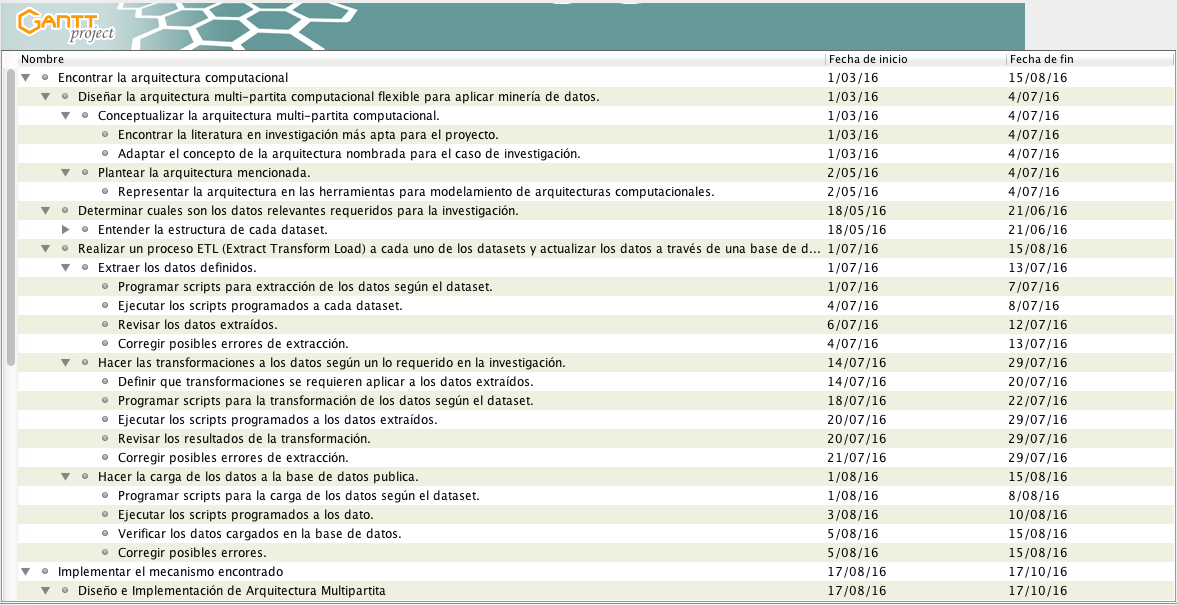
\includegraphics[width=\textwidth]{Imagen1.png}
\end{center}
\end{sidewaystable}
\clearpage

\begin{sidewaystable}
\begin{center}
Parte 2
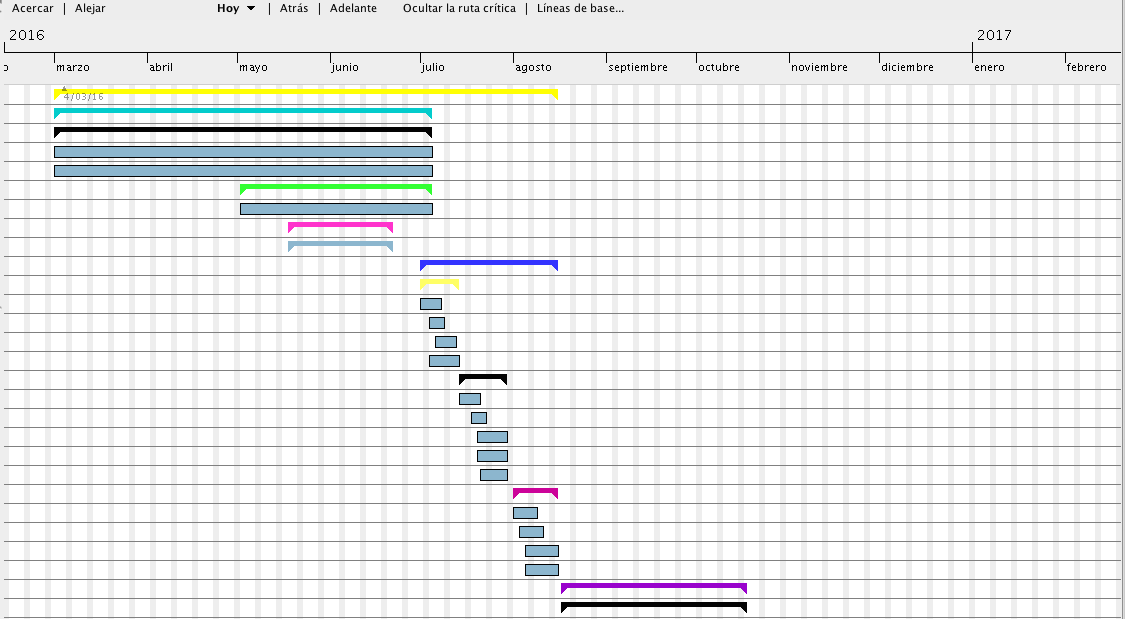
\includegraphics[width=\textwidth]{Imagen3.png}
\end{center}
\end{sidewaystable}
\clearpage

\begin{sidewaystable}
\begin{center}
Parte 3
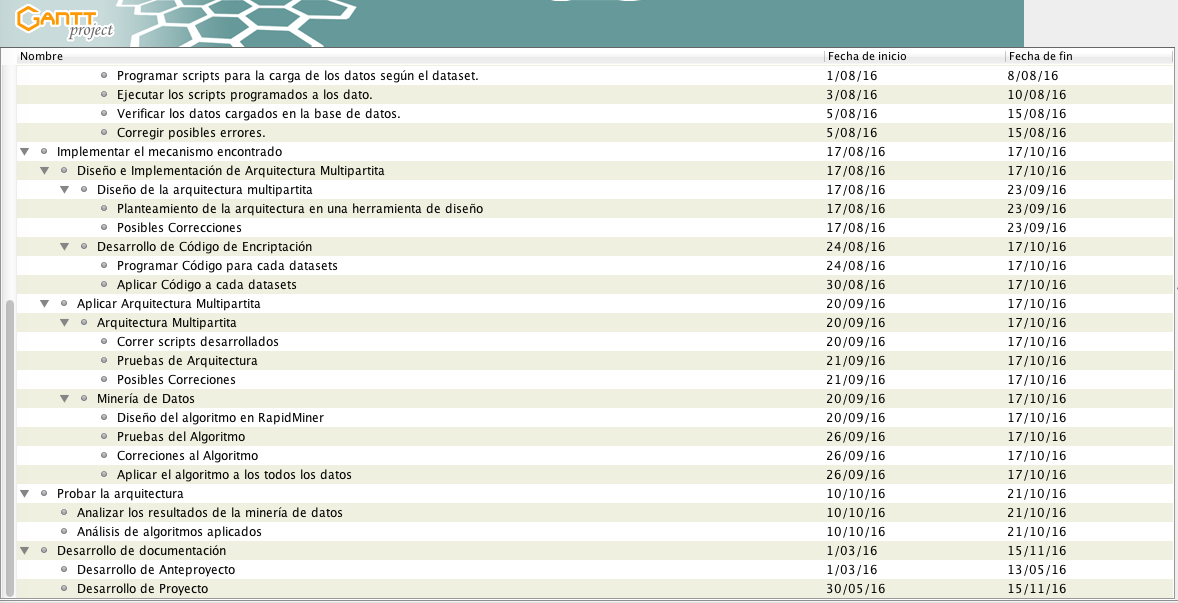
\includegraphics[width=\textwidth]{Imagen2.png}
\end{center}
\end{sidewaystable}
\clearpage

\begin{sidewaystable}
\begin{center}
Parte 4
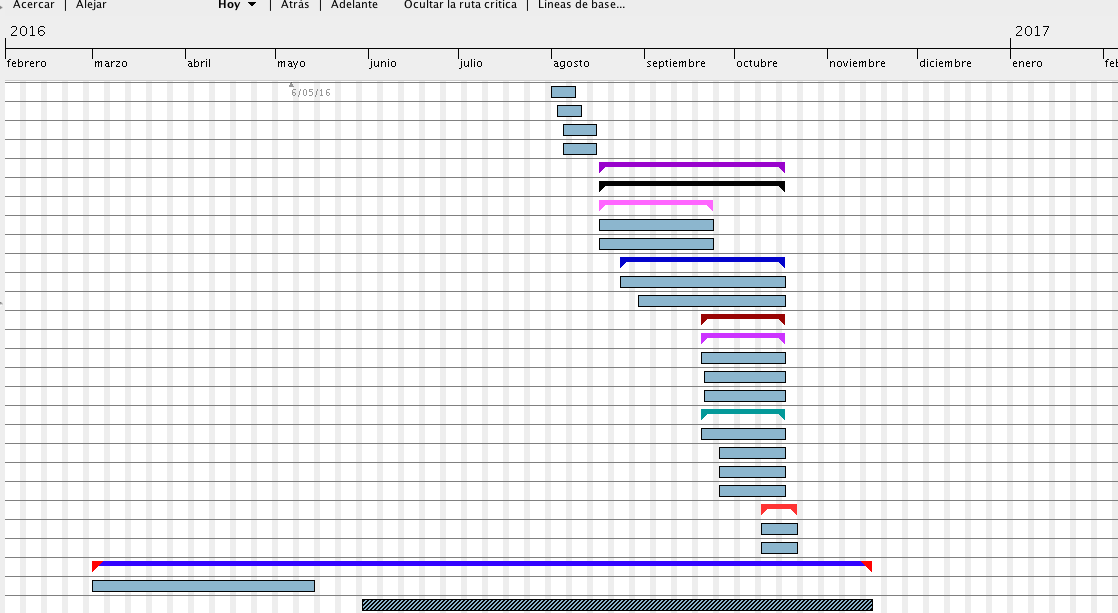
\includegraphics[width=\textwidth]{Imagen4.png}
\end{center}
\end{sidewaystable}
\clearpage

\begin{sidewaystable}
\begin{center}
\section{RECURSOS}
\end{center}
\begin{center}
Parte 1
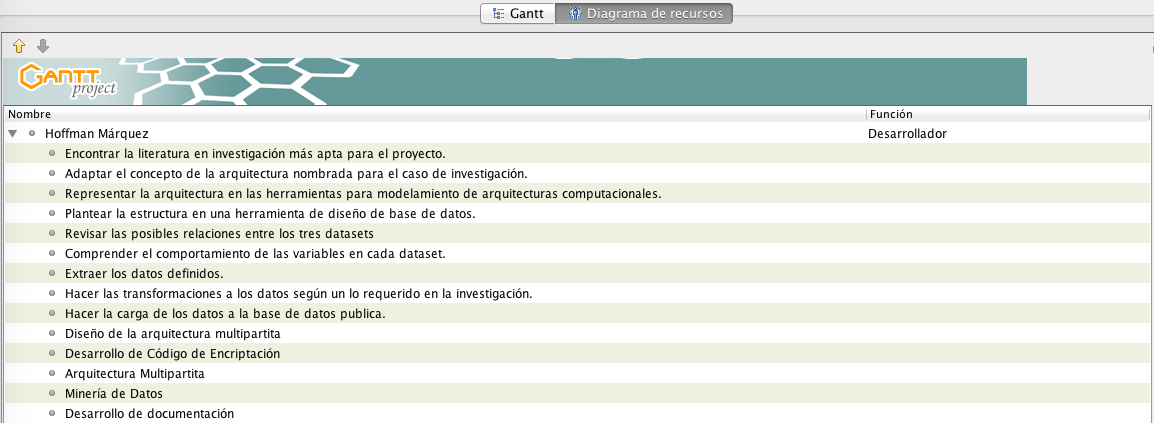
\includegraphics[width=\textwidth]{Hoffman1.png}
\end{center}
\end{sidewaystable}
\clearpage

\begin{sidewaystable}
\begin{center}
Parte 2
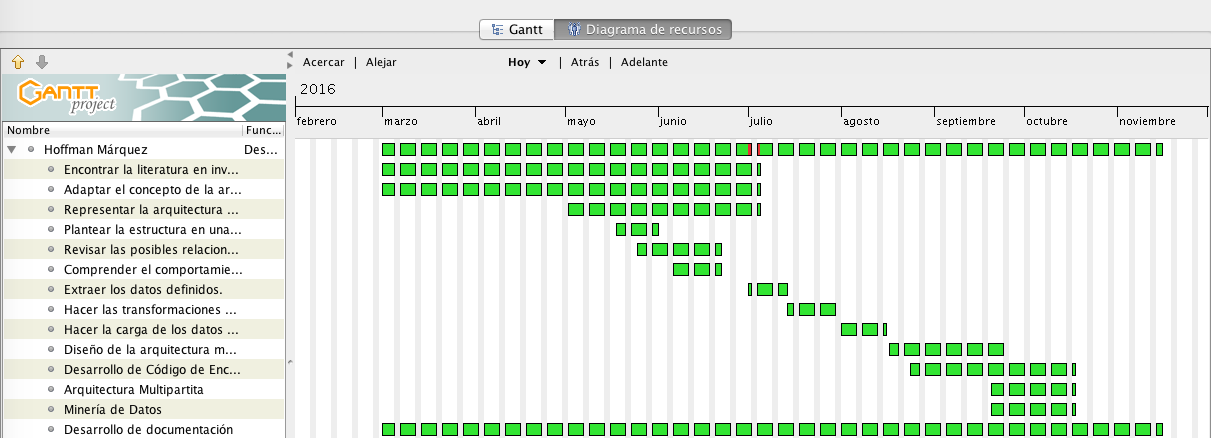
\includegraphics[width=\textwidth]{Hoffma2.png}
\end{center}
\end{sidewaystable}
\clearpage

\begin{sidewaystable}
\begin{center}
Parte 3
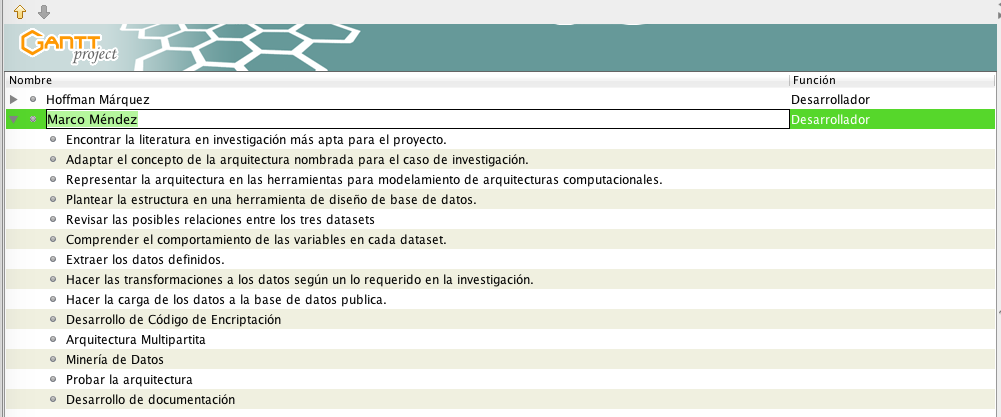
\includegraphics[width=\textwidth]{Marco1.png}
\end{center}
\end{sidewaystable}
\clearpage

\begin{sidewaystable}
\begin{center}
Parte 4
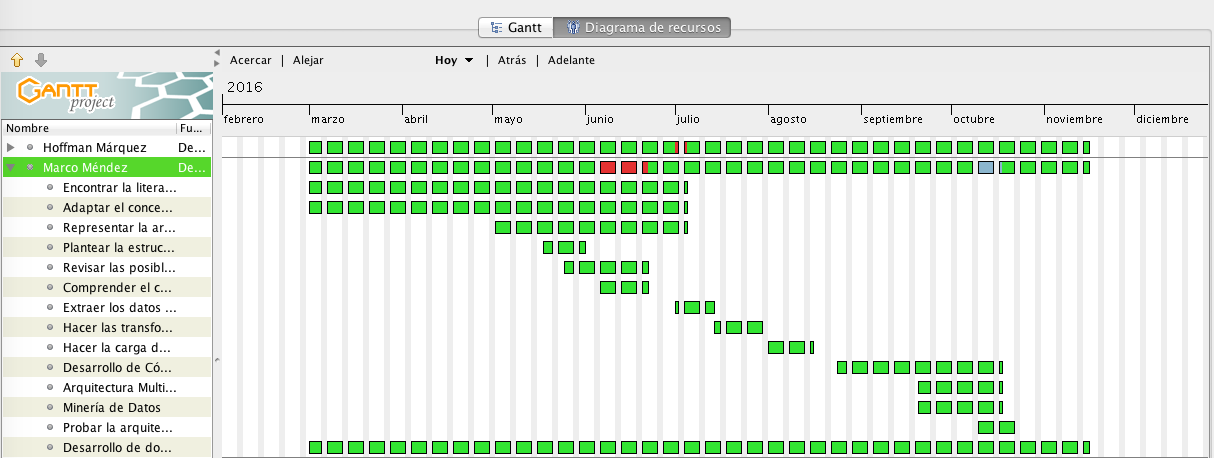
\includegraphics[width=\textwidth]{Marco2.png}
\end{center}
\end{sidewaystable}
\clearpage

\clearpage



% Bibliografa.
%-----------------------------------------------------------------

\begin{thebibliography}{99}

\bibitem[1]{R. O. Duda.}DR. O. Duda.\emph{P. E. Hart, and D. Stork, “Pattern Classification”, 2001, Wiley series in Probabilistic and Statistic, John Wiley and Sons, Second Edition.}

\bibitem[2]{G. Karypis.} G. Karypis.\emph{E. H. Han. And V. Kumar, “Chameleon: A hierarchical clustering algorithm using dynamic modeling”, IEEE Computer, 1999, 32(8), pag. 68-75.}

\bibitem[3]{T. Zhang, R. Ramakrishnan, and M. Livny.}T. Zhang, R. Ramakrishnan, and M. Livny.\emph{“BIRCH: An efficient data Clustering method for very large databases”, In Proceedings of ACM SIGMOD Conference on Management of Data, 1996, pag. 103-114.}

\bibitem[4]{S. Guha, R. Rastogi, and K. Shim,}S. Guha, R. Rastogi, and K. Shim,\emph{“CURE: An efficient clustering algorithm for large databases”, In Proceedings of ACM SIGMOD 98, 1998, pag. 73- 84.}

\bibitem[5]{M. Ester, H.P. Kriegel, J. Sander and X. Xu.}M. Ester, H.P. Kriegel, J. Sander and X. Xu.\emph{“A density-based algorithm for discovering clusters in large spatial databases with noise”, In Proceedings of International Conference on Knoowledge Discovery and Data Mining (KDD 96), 1996, pag 226-231.}

\bibitem[6]{M. Ankerst, M. Bruenig, H. P. Kriegel, and J. Sander.}M. Ankerst, M. Bruenig, H. P. Kriegel, and J. Sander\emph{“OPTICS: ordering points tu identify the clustering structure”, In Proceedings of ACM SIGMOD International Conference on Management of Data, 1999, pag. 49- 60.}

\bibitem[7]{Thanh N. Tran.}Thanh N. Tran.\emph{“Knn Density-Based Clustering for High Dimensional Multispectral Images”.}

\bibitem[8]{L. Ertoz, M. Steinbach.}L. Ertoz, M. Steinbach.\emph{V. Kumar, “Finding Clusters of Different Sizes, Shapes and Densities in Noise”, 2003,}

\bibitem[9]{] A. Hinneburg, and D. A. Keim.}] A. Hinneburg, and D. A. Keim.\emph{“An efficient Approach to Clustering in Large Multimedia Databases with Noise”, in Proceedings Knowledge Discovery and Data Mining, 1998, pag. 58-65.}

%Agrupamiento Clustering Referencias

\bibitem[10]{DAN Goodin.}DAN Goodin.\emph{Poorly anonymized logs reveal NYC cab drivers’ detailed whereabouts [En linea]. New York: Dirección URL: <http://arstechnica.com/tech-policy/2014/06/poorly-anonymized-logs-reveal-nyc-cab-drivers-detailed-whereabouts/>. [30, Marzo 2015].}

\bibitem[11]{HERNANDEZ ALEXANDER.}HERNANDEZ ALEXANDER.\emph{New York taxi details can be extracted from anonymised data, researchers say [En linea]. New York: Dirección URL: <https://www.theguardian.com/technology/2014/jun/27/new-york-taxi-details-anonymised-data-researchers-warn>. [30, Marzo 2015].}

\bibitem[12]{HERRANZ Javier NIN Jordi.}HERRANZ Javier , NIN Jordi.\emph{Secure and efficient anonymization of distributed confidential databases, Springer-Verlag Berlin Heidelberg 2014, Online: 23 April 2014. Int. J. Inf. Secur. (2014) 13:497–512, Pág 4.}

\bibitem[13]{DAMGARD Ivan, PASTRO Valerio, SMART Nigel, ZAKARIAS Sarah .}DAMGARD Ivan, PASTRO Valerio, SMART Nigel, ZAKARIAS Sarah .\emph{Multiparty Computation from Somewhat Homomorphic Encryption, International Association for Cryptologic Research 2012, R. Safavi-Naini and R. Canetti (Eds.): CRYPTO 2012, LNCS 7417, pp. 643.}

\bibitem[14]{GHODOSI Hossein Ghodosi, PIEPRZYK Josef, STEINFELD Ron.}GHODOSI Hossein Ghodosi, PIEPRZYK Josef, STEINFELD Ron .\emph{Multi-party computation with conversion of secret sharing, Springer Science+Business Media, LLC 2011, Des. Codes Cryptogr. (2012) 62:259–272, Online: 10 May 2011,pp. 260.}

\bibitem[15]{KIRAZ SABIR Mehmet, UZUNKOL Osmanbey.}KIRAZ SABIR Mehmet, UZUNKOL Osmanbey .\emph{Efficient and verifiable algorithms for secure outsourcing of cryptographic computations, Springer-Verlag Berlin Heidelberg 2015, Int. J. Inf. Secur, Online: 15 Nov 2015,pp. 1.}

\bibitem[16]{LAUD Peeter.}LAUD Peeter .\emph{Privacy-Preserving Minimum Spanning Trees through Oblivious Parallel RAM for Secure Multiparty Computation, Online: 25 Nov 2014,pp. 3.}

\bibitem[17]{LAUD Peeter.}LAUD Peeter .\emph{Privacy-Preserving Minimum Spanning Trees through Oblivious Parallel RAM for Secure Multiparty Computation, Online: 25 Nov 2014,pp. 5.}

\bibitem[18]{GAITAN Mauricio, CANCINO Juliana, BEHRENTZ Eduardo.} GAITAN Mauricio, CANCINO Juliana, BEHRENTZ Eduardo .\emph{Análisis del estado de la calidad del aire en Bogotá, Online: 1 OCT 2007,pp. 3.}

\bibitem[19]{CORREAL Maria Elsa Correal, MARTHA Juan Esteban, SARMIENTO Rodrigo.} GCORREAL María Elsa Correal, MARTHÁ Juan Esteban, SARMIENTO Rodrigo .\emph{Influencia de la variabilidad climática en las enfermedades respiratorias agudas en Bogotá, 2013, Biomédica 2015;35(Supl.2):130-8, <http://dx.doi.org/10.7705/biomedica.v35i0.2456> , pp. 131.}

\bibitem[20]{CORREAL Maria Elsa Correal, MARTHA Juan Esteban, SARMIENTO Rodrigo.} GCORREAL María Elsa Correal, MARTHÁ Juan Esteban, SARMIENTO Rodrigo .\emph{Influencia de la variabilidad climática en las enfermedades respiratorias agudas en Bogotá, 2013, Biomédica 2015;35(Supl.2):130-8, <http://dx.doi.org/10.7705/biomedica.v35i0.2456> , pp. 131.}

\bibitem[21]{CORREAL Maria Elsa Correal, MARTHA Juan Esteban, SARMIENTO Rodrigo.} GCORREAL María Elsa Correal, MARTHÁ Juan Esteban, SARMIENTO Rodrigo .\emph{Influencia de la variabilidad climática en las enfermedades respiratorias agudas en Bogotá, 2013, Biomédica 2015;35(Supl.2):130-8, <http://dx.doi.org/10.7705/biomedica.v35i0.2456> , pp. 133.}

\bibitem[22]{KIRAZ SABIR Mehmet, UZUNKOL Osmanbey.}KIRAZ SABIR Mehmet, UZUNKOL Osmanbey .\emph{Efficient and verifiable algorithms for secure outsourcing of cryptographic computations, Springer-Verlag Berlin Heidelberg 2015, Int. J. Inf. Secur, Online: 15 Nov 2015,pp. 2.}

\bibitem[23]{KIRAZ SABIR Mehmet, UZUNKOL Osmanbey.}KIRAZ SABIR Mehmet, UZUNKOL Osmanbey .\emph{Efficient and verifiable algorithms for secure outsourcing of cryptographic computations, Springer-Verlag Berlin Heidelberg 2015, Int. J. Inf. Secur, Online: 15 Nov 2015,pp. 4.}

\bibitem[24]{GHODOSI Hossein Ghodosi, PIEPRZYK Josef, STEINFELD Ron.}GHODOSI Hossein Ghodosi, PIEPRZYK Josef, STEINFELD Ron .\emph{Multi-party computation with conversion of secret sharing, Springer Science+Business Media, LLC 2011, Des. Codes Cryptogr. (2012) 62:259–272, Online: 10 May 2011,pp. 263.}

\end{thebibliography}
\end{document}